\begin{figure*}[t]
\centering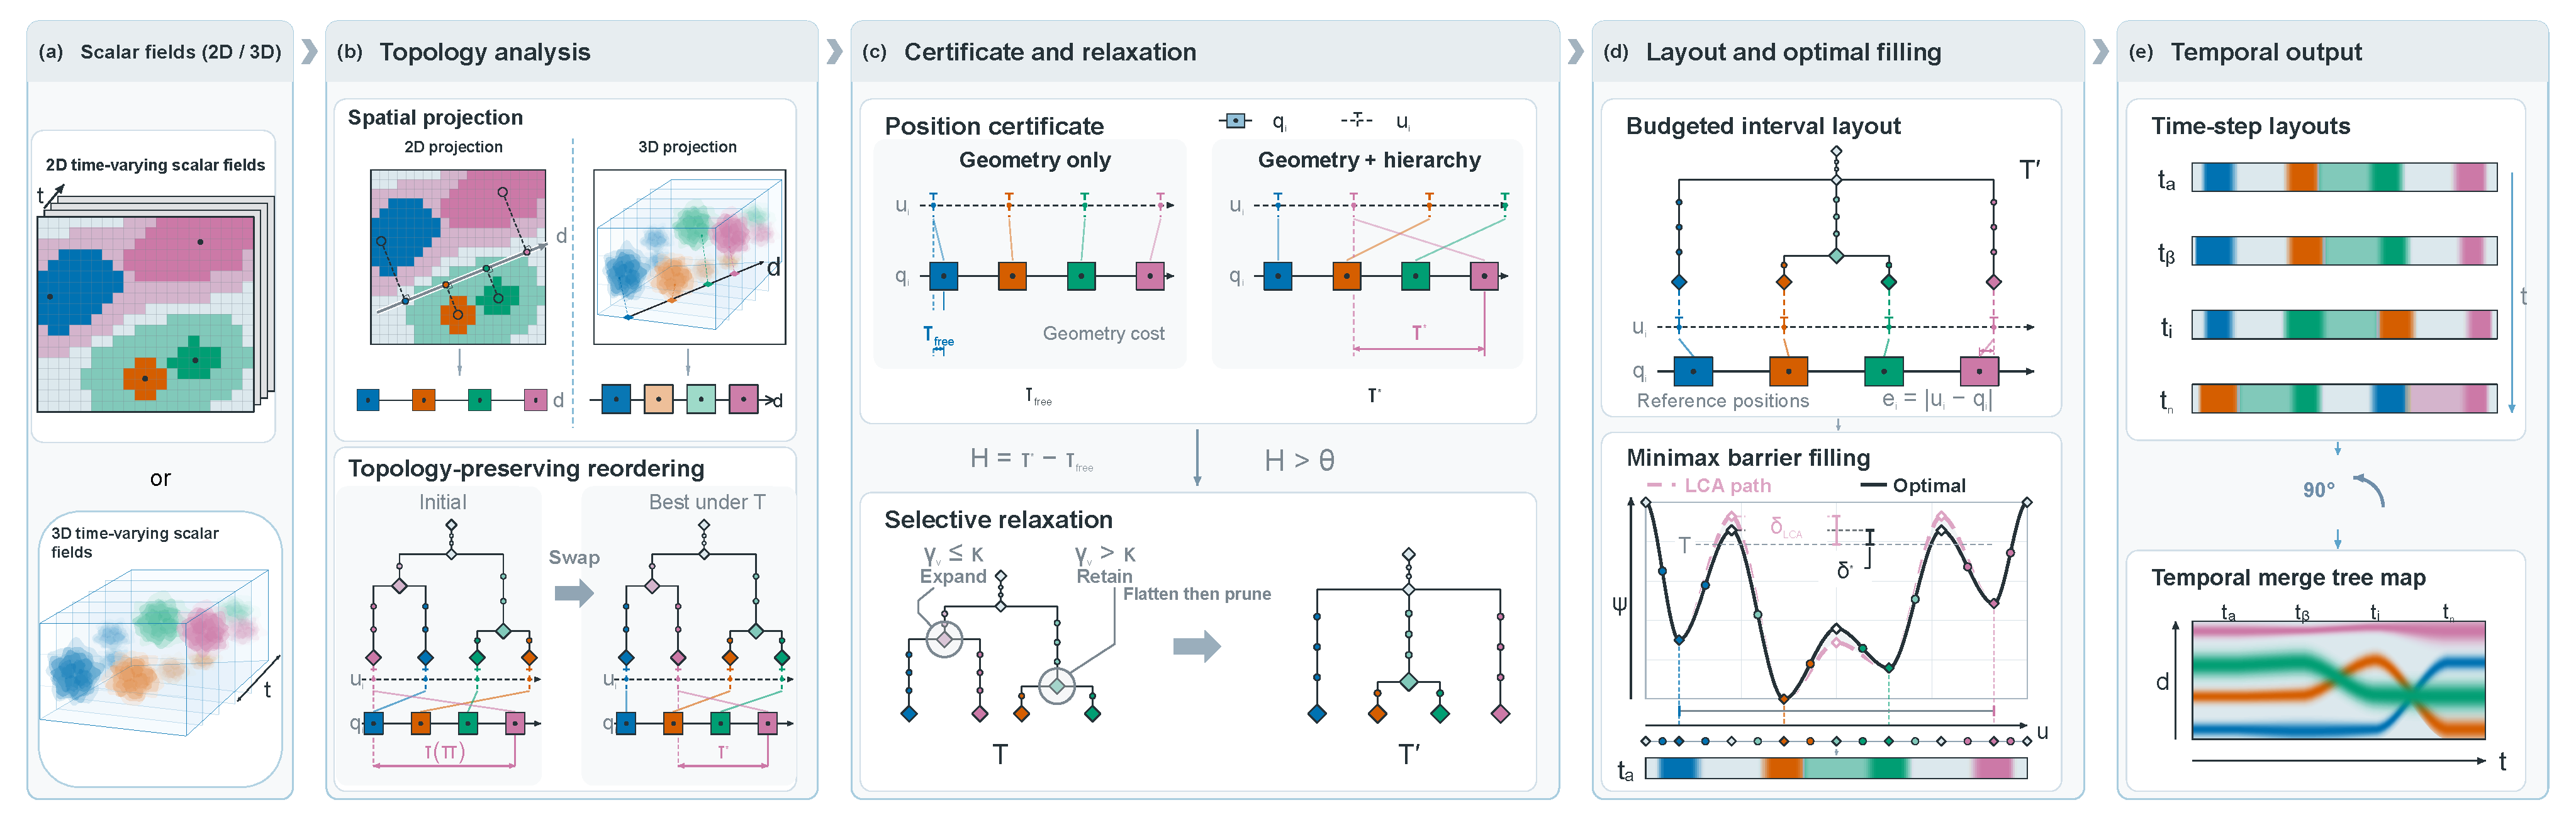
\includegraphics[width=\textwidth]{figures/Fig3.pdf}
\caption{RG-MTM's five stages (a)--(e), using the supplied four-feature schematic. Trees and a fixed projection define source merge targets and reference positions. Certificates diagnose hierarchy-dependent displacement; selective relaxation expands the ordering tree. Budgeted intervals and minimax filling construct profiles, stacked through time. The four branch identities retain blue, orange, green, and purple across stages; actual maps encode scalar values. Flatten-then-prune restoration is used in the planar protocol. $\kappa$ controls eligibility; output barriers determine measured cost.}
\label{fig:pipeline}
\end{figure*}
